\documentclass[
  12pt,
  openright,
  oneside,
  a4paper,
  english,
  brazil
]{abntex2}


\newcommand{\nomeInstituicao}{FATEC MARÍLIA}
\newcommand{\nomeCurso}{DESENVOLVIMENTO DE SOFTWARE MULTIPLATAFORMA}
\newcommand{\nomeDisciplina}{LABORATÓRIO DE DESENVOLVIMENTO MOBILE}
\newcommand{\nomeProfessor}{Prof. Luiz Carlos Querino Filho}
\newcommand{\nomeAluno}{Marcos Daniel da Silva Lima}
\newcommand{\cidadeTrabalho}{Marília, SP}

% ----------------------------------------------------------
% Pacotes e configuração ABNT
% ----------------------------------------------------------
\usepackage[utf8]{inputenc}
\usepackage[T1]{fontenc}
\usepackage{lmodern}
\usepackage{microtype}
\usepackage{graphicx}
\usepackage{booktabs}
\usepackage{tabularx}
\usepackage{array}
\usepackage{enumitem}
\usepackage{float}\usepackage{pdflscape}
\usepackage{xcolor}
\usepackage{tikz}
\usetikzlibrary{arrows.meta,positioning,shapes.geometric}
\usepackage[alf]{abntex2cite}
\usepackage{hyperref}
\usepackage{url}

\definecolor{agendteal}{HTML}{008FA3}
\definecolor{agendlight}{HTML}{E8F7F9}\definecolor{agendgray}{HTML}{F3F6F7}

\hypersetup{
  colorlinks=true,
  linkcolor=black,
  citecolor=black,
  urlcolor=agendteal,
  pdftitle={Agend.AI Profissional — Relatório de Projeto de Laboratório},
  pdfauthor={\nomeAluno}
}

\setlrmarginsandblock{3cm}{2cm}{*}
\setulmarginsandblock{3cm}{2cm}{*}
\checkandfixthelayout
\setlength{\parindent}{1.25cm}
\setlength{\parskip}{0pt}
\OnehalfSpacing

\renewcommand{\arraystretch}{1.25}
\newcolumntype{Y}{>{\raggedright\arraybackslash}X}
\newcolumntype{C}[1]{>{\centering\arraybackslash}p{#1}}

% ----------------------------------------------------------
% Informações do trabalho
% ----------------------------------------------------------
\titulo{AGEND.AI PROFISSIONAL: APLICATIVO MOBILE DE AUTOGESTÃO PROFISSIONAL}
\autor{\nomeAluno}
\local{\cidadeTrabalho}
\data{2026}
\instituicao{%
  \nomeInstituicao
  \par
  \nomeCurso
  \par
  \nomeDisciplina
}
\tipotrabalho{Relatório de projeto}
\preambulo{Relatório apresentado à disciplina \nomeDisciplina, ministrada por \nomeProfessor, como parte da avaliação do projeto mobile.}

\begin{document}
\selectlanguage{brazil}
\frenchspacing

\pretextual
\imprimircapa
\imprimirfolhaderosto*

\pdfbookmark[0]{\contentsname}{toc}
\tableofcontents*
\cleardoublepage

\textual

% ==========================================================
\chapter{Definição do problema}
% ==========================================================

\section{Contexto, justificativa e objetivos}

Profissionais que atendem em clínicas dependem da agenda institucional para organizar consultas e procedimentos, mas nem sempre possuem uma visão simples e centralizada da própria rotina. Informações sobre compromissos, horários indisponíveis, serviços oferecidos, preços e previsão de receitas podem ficar distribuídas entre sistemas administrativos, calendários e contatos com a recepção.

O \textbf{Agend.AI Profissional} será um aplicativo de autogestão integrado ao sistema da clínica. Seu objetivo é oferecer ao profissional uma visão individual da rotina, sem substituir o sistema administrativo. A primeira versão permitirá consultar a agenda, bloquear horários, visualizar um resumo de receitas e administrar os procedimentos oferecidos.

\section{Público-alvo}

O aplicativo será destinado a profissionais de saúde e bem-estar vinculados a clínicas que utilizam o Agend.AI, como médicos, psicólogos, fisioterapeutas, nutricionistas e profissionais de estética. O uso ocorrerá pelo celular, entre atendimentos ou fora da clínica. Administradores e recepcionistas continuarão utilizando a aplicação Web, enquanto os clientes realizarão agendamentos pelos canais da clínica e pelo chatbot.

\section{Análise de similares}

Foram analisadas duas soluções já consolidadas no mercado.

\begin{table}[H]
\centering
\caption{Comparação com aplicativos similares}
\small
\begin{tabularx}{\textwidth}{p{2.4cm}YY}
\toprule
\textbf{Solução} & \textbf{Recursos observados} & \textbf{Relação com o Agend.AI Profissional} \\
\midrule
iClinic & Agenda médica, bloqueio de horários, procedimentos com duração e valor, sincronização com calendários e gestão financeira \cite{iclinic2026}. & É uma solução ampla de gestão clínica. O Agend.AI adota um recorte menor e centrado na autonomia do profissional. \\
\addlinespace
Doctoralia Pro & Agendamento on-line, lembretes automáticos, comunicação com pacientes e ferramentas de visibilidade profissional \cite{doctoralia2026}. & Possui forte foco na captação de pacientes. O Agend.AI prioriza a integração com a operação interna da clínica. \\
\bottomrule
\end{tabularx}
\end{table}

Os diferenciais propostos são a integração com o catálogo da clínica, a personalização de preço e duração por profissional e o uso do Google Calendar por meio do n8n. Dessa forma, o aplicativo permanece simples e conectado ao restante do ecossistema Agend.AI.

\section{Definição do MVP}

O Produto Mínimo Viável será composto por cinco grupos de recursos essenciais:

\begin{enumerate}[label=\arabic*.]
  \item autenticação do profissional e consulta do próprio perfil;
  \item visualização da agenda e dos detalhes de um atendimento;
  \item criação e remoção de indisponibilidades pontuais;
  \item resumo de receitas realizadas e previstas;
  \item seleção de procedimentos do catálogo da clínica e alteração de preço, duração e disponibilidade.
\end{enumerate}

Não farão parte desta entrega: reagendamento pelo Telegram, notificações push, recuperação de senha, indisponibilidades recorrentes, criação de novos procedimentos pelo profissional e detalhamento financeiro por atendimento. Esses recursos poderão ser avaliados após a validação do MVP.

% ==========================================================
\chapter{Design de experiência e interface — UX/UI}
% ==========================================================

\section{Fluxograma do usuário}

A Figura~\ref{fig:userflow} representa o fluxo principal desde a abertura do aplicativo até a conclusão de uma tarefa.

\begin{figure}[H]
\centering
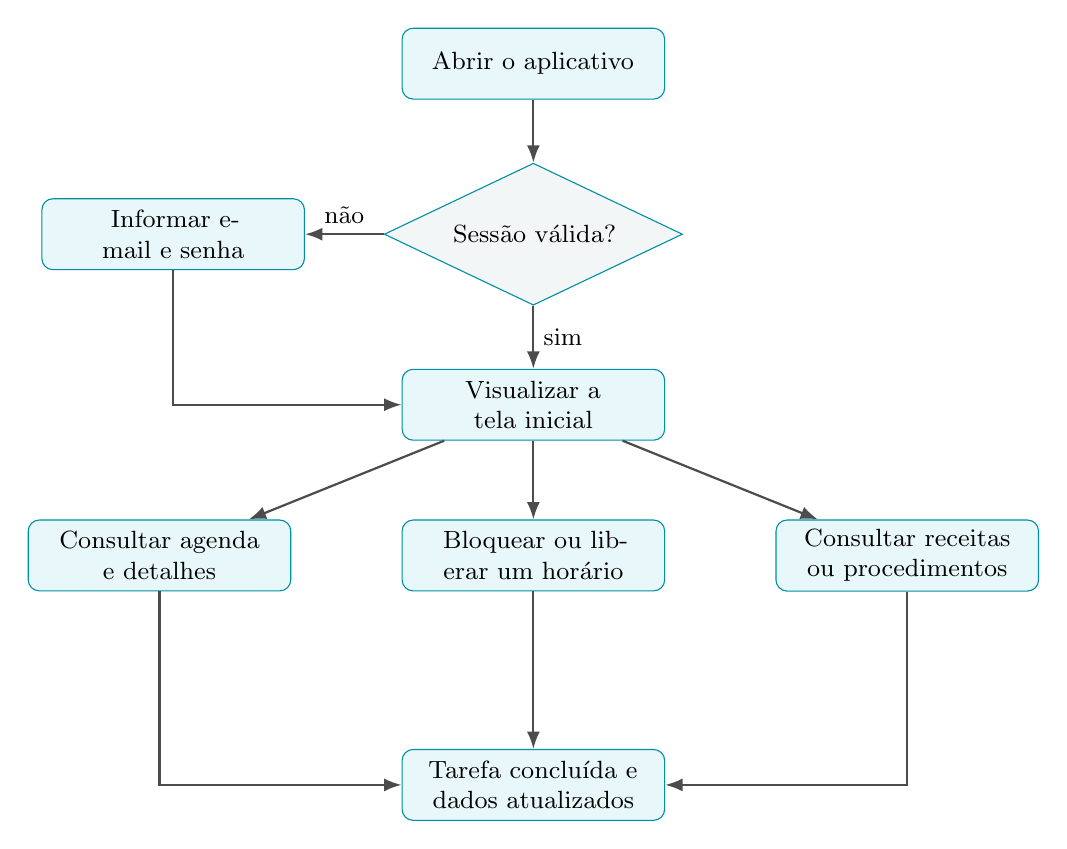
\begin{tikzpicture}[
  node distance=0.8cm and 1.0cm,
  every node/.style={font=\small},
  etapa/.style={rectangle, rounded corners, draw=agendteal, fill=agendlight, minimum height=0.9cm, text width=3.1cm, align=center},
  decisao/.style={diamond, aspect=2.1, draw=agendteal, fill=agendgray, text width=2.6cm, align=center},
  seta/.style={-{Latex[length=2.2mm]}, thick, draw=black!70}
]
  \node[etapa] (abrir) {Abrir o aplicativo};
  \node[decisao, below=of abrir] (sessao) {Sessão válida?};
  \node[etapa, left=of sessao] (login) {Informar e-mail e senha};
  \node[etapa, below=of sessao] (inicio) {Visualizar a tela inicial};
  \node[etapa, below left=1cm and 1.4cm of inicio] (agenda) {Consultar agenda e detalhes};
  \node[etapa, below=1cm of inicio] (bloqueio) {Bloquear ou liberar um horário};
  \node[etapa, below right=1cm and 1.4cm of inicio] (gestao) {Consultar receitas ou procedimentos};
  \node[etapa, below=2.0cm of bloqueio] (fim) {Tarefa concluída e dados atualizados};

  \draw[seta] (abrir) -- (sessao);
  \draw[seta] (sessao) -- node[right]{sim} (inicio);
  \draw[seta] (sessao) -- node[above]{não} (login);
  \draw[seta] (login) |- (inicio);
  \draw[seta] (inicio) -- (agenda);
  \draw[seta] (inicio) -- (bloqueio);
  \draw[seta] (inicio) -- (gestao);
  \draw[seta] (agenda) |- (fim);
  \draw[seta] (bloqueio) -- (fim);
  \draw[seta] (gestao) |- (fim);
\end{tikzpicture}
\caption{Fluxo principal do usuário}
\label{fig:userflow}
\end{figure}

\section{Wireframes de baixa fidelidade}

Os wireframes abaixo representam a estrutura das três telas centrais. Na implementação, o conteúdo manterá margem lateral aproximada de 20 pontos e controles com área de toque mínima próxima de 44 por 44 pontos.

\begin{figure}[H]
\centering
\setlength{\fboxsep}{7pt}
\fbox{\begin{minipage}[t][6.7cm][t]{0.27\textwidth}
\centering\textbf{Início}\par\vspace{0.3cm}
\raggedright\small
[ Saudação e perfil ]\\[0.25cm]
[ Resumo de receitas ]\\[0.25cm]
[ Próximo atendimento ]\\[1cm]
\hrule\vspace{0.15cm}
Início \quad Agenda \quad Perfil
\end{minipage}}
\hfill
\fbox{\begin{minipage}[t][6.7cm][t]{0.27\textwidth}
\centering\textbf{Agenda}\par\vspace{0.3cm}
\raggedright\small
[ Semana / data ]\\[0.25cm]
[ 08:00 Atendimento ]\\[0.25cm]
[ 10:30 Atendimento ]\\[0.25cm]
[ 12:00 Indisponível ]\\[0.6cm]
[ + Bloquear horário ]
\end{minipage}}
\hfill
\fbox{\begin{minipage}[t][6.7cm][t]{0.27\textwidth}
\centering\textbf{Procedimentos}\par\vspace{0.3cm}
\raggedright\small
[ Procedimento ativo ]\\
Valor \quad Duração\\[0.25cm]
[ Procedimento ativo ]\\
Valor \quad Duração\\[0.4cm]
[ Adicionar do catálogo ]
\end{minipage}}
\caption{Wireframes de baixa fidelidade}
\label{fig:wireframes}
\end{figure}

\section{Protótipo de alta fidelidade}

O protótipo foi desenvolvido no Figma com a identidade visual do Agend.AI, navegação inferior e telas em formato 390 por 844 pontos. A Figura~\ref{fig:prototipo} apresenta a board visual. O arquivo interativo está disponível em \href{https://www.figma.com/design/3qnRyQzajwSLsqfhsBw8Vw/Agend.AI?node-id=186-2&t=8hZQjo2DGDWcCZ2N-1}{Agend.AI — página App}.

\begin{figure}[H]
\centering
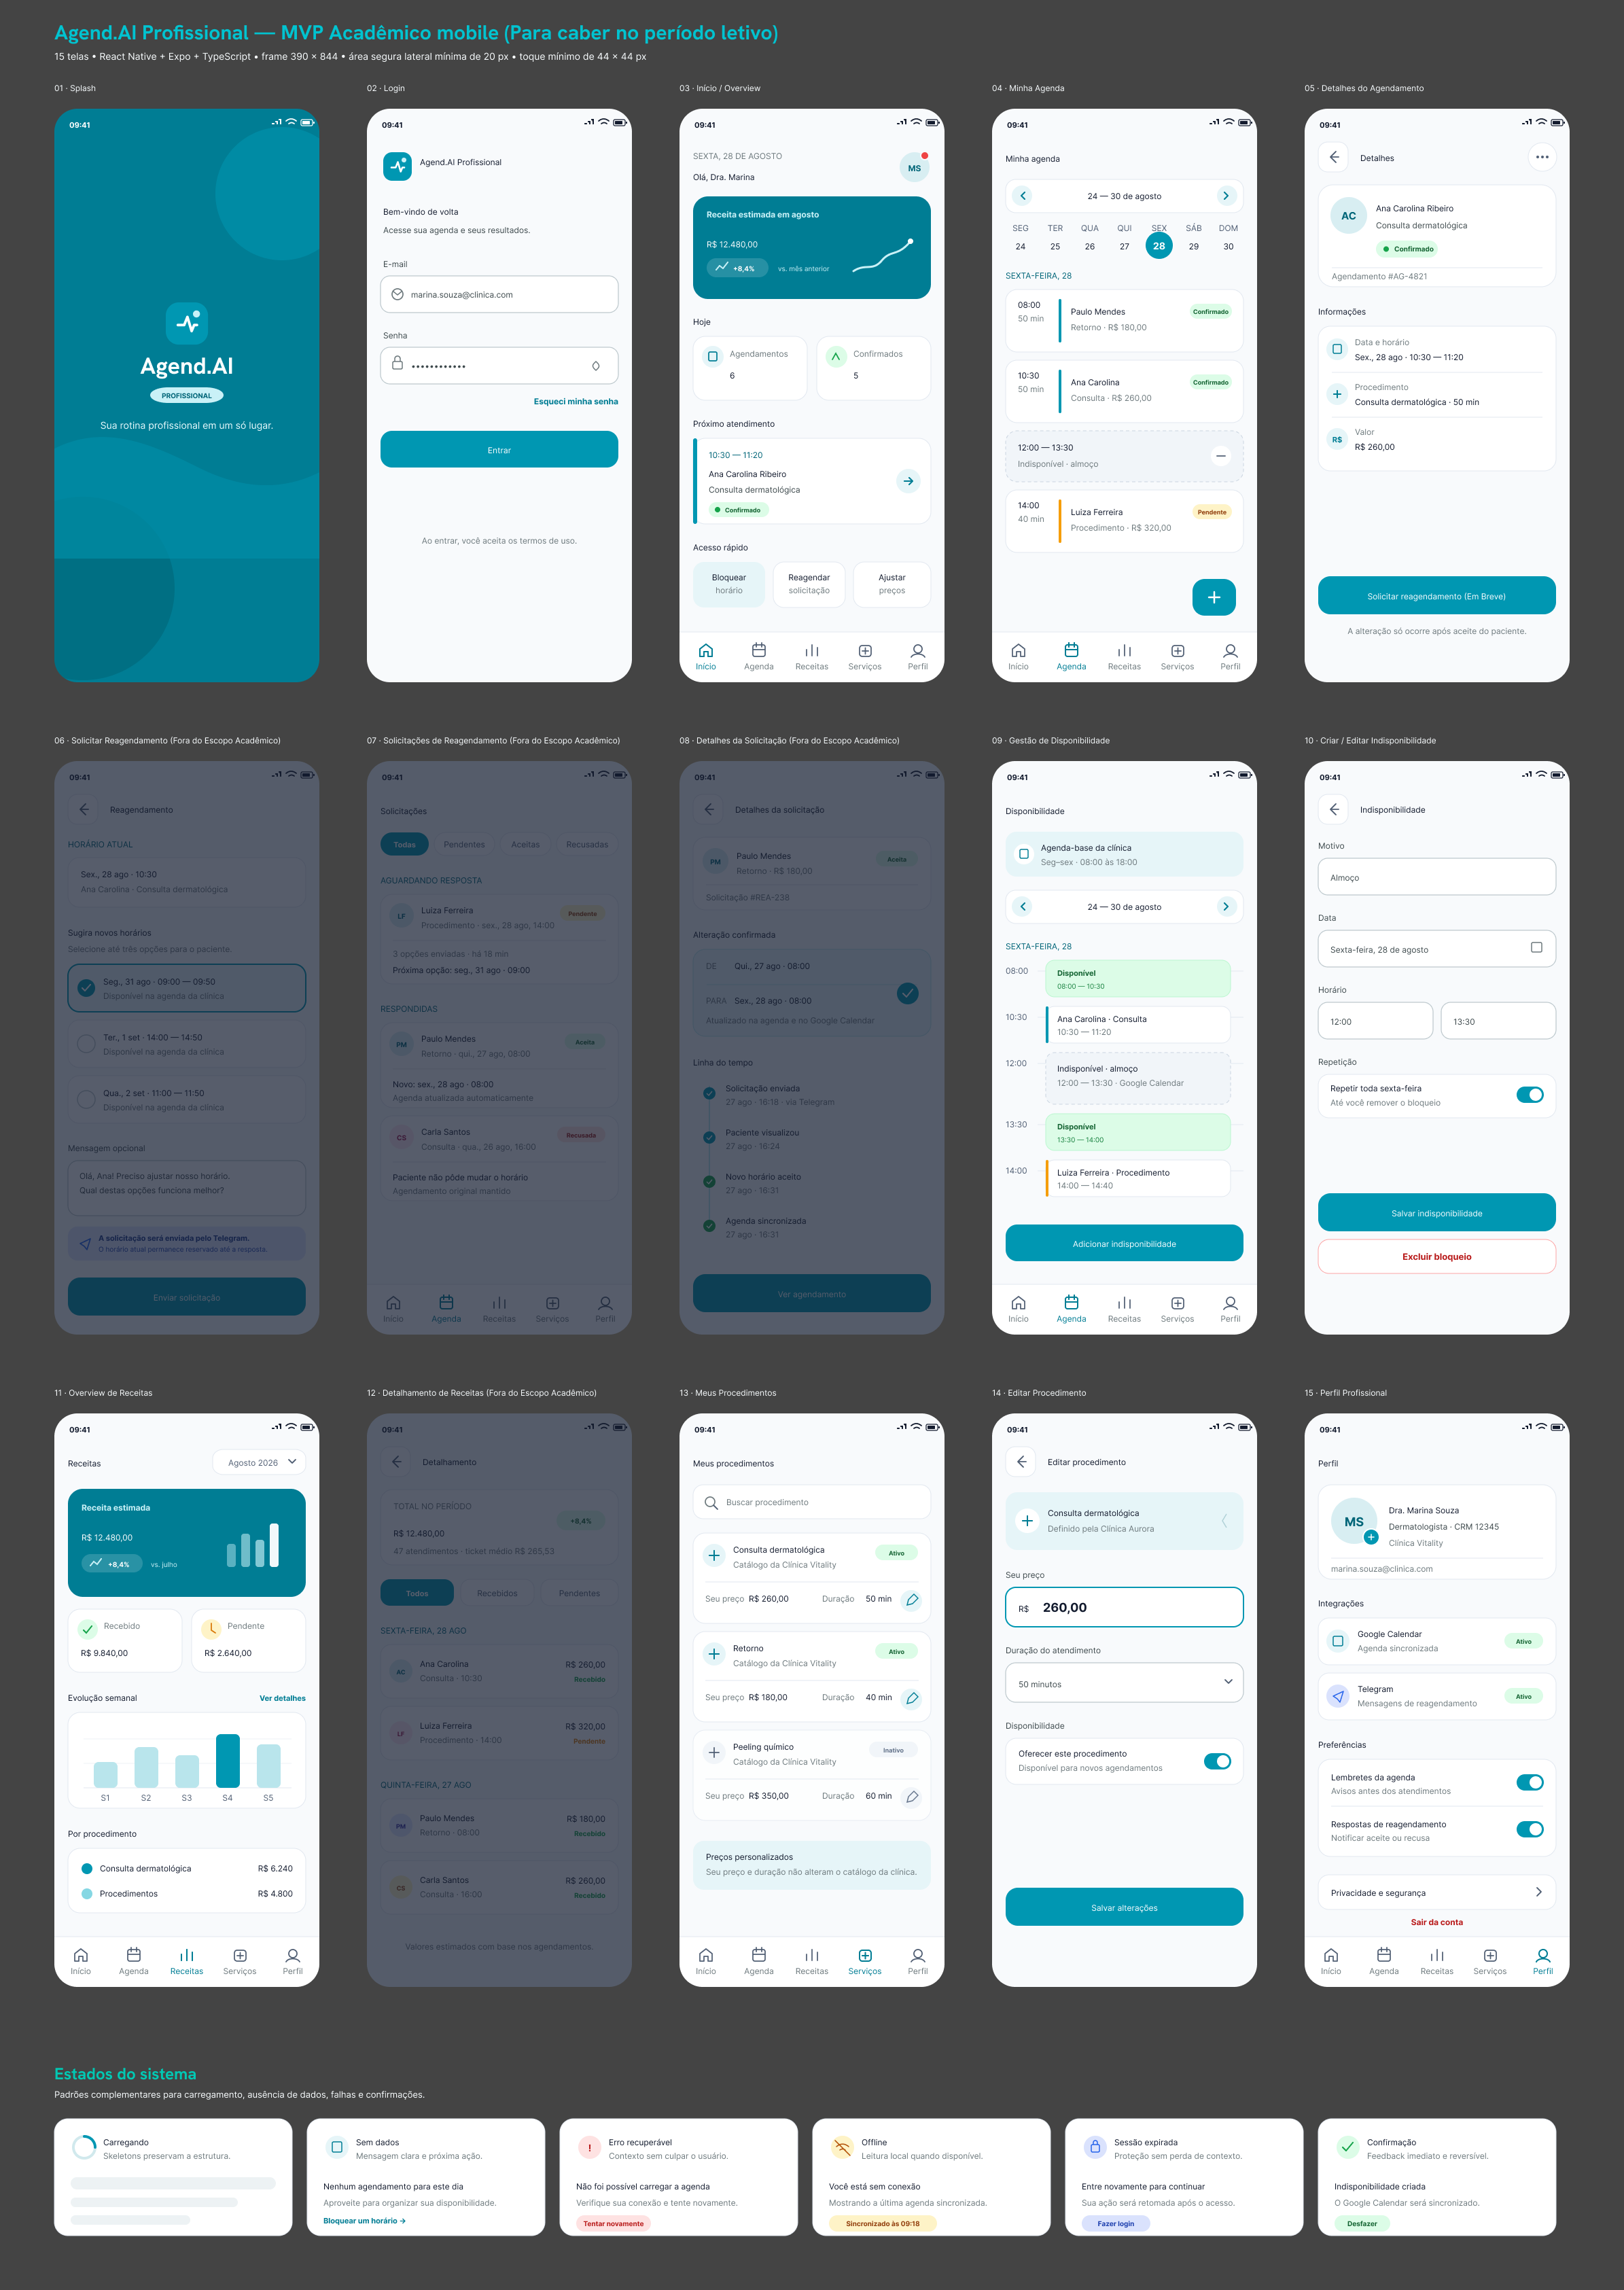
\includegraphics[width=0.93\textwidth,height=0.70\textheight,keepaspectratio]{assets/prototipo-figma.png}
\caption{Board do protótipo de alta fidelidade}
\label{fig:prototipo}
\end{figure}

A board registra também estudos de funcionalidades futuras. Para o MVP acadêmico serão consideradas apenas as telas de autenticação, início, agenda, detalhes, disponibilidade, receitas resumidas, procedimentos e perfil.

% ==========================================================
\chapter{Arquitetura técnica e modelagem}
% ==========================================================

\section{Tecnologia escolhida}

A aplicação será desenvolvida com \textbf{React Native, Expo e TypeScript}. O React Native permite criar interfaces nativas para Android e iOS utilizando o modelo de componentes do React \cite{reactnative2026}. O Expo complementa essa tecnologia com ferramentas de desenvolvimento, navegação e geração de builds a partir de um único projeto TypeScript \cite{expo2026}.

A escolha se justifica pelo prazo acadêmico, pelo reaproveitamento do conhecimento já aplicado no frontend Web em React e pela possibilidade de manter uma única base de código para as duas plataformas. TypeScript acrescenta verificação estática de tipos, reduzindo erros na comunicação com a API.

\section{Diagrama de entidade-relacionamento}

O MER da Figura~\ref{fig:der} apresenta as entidades diretamente relacionadas ao escopo acadêmico, seus relacionamentos e suas cardinalidades.\begin{landscape}\begin{figure}[H]\centering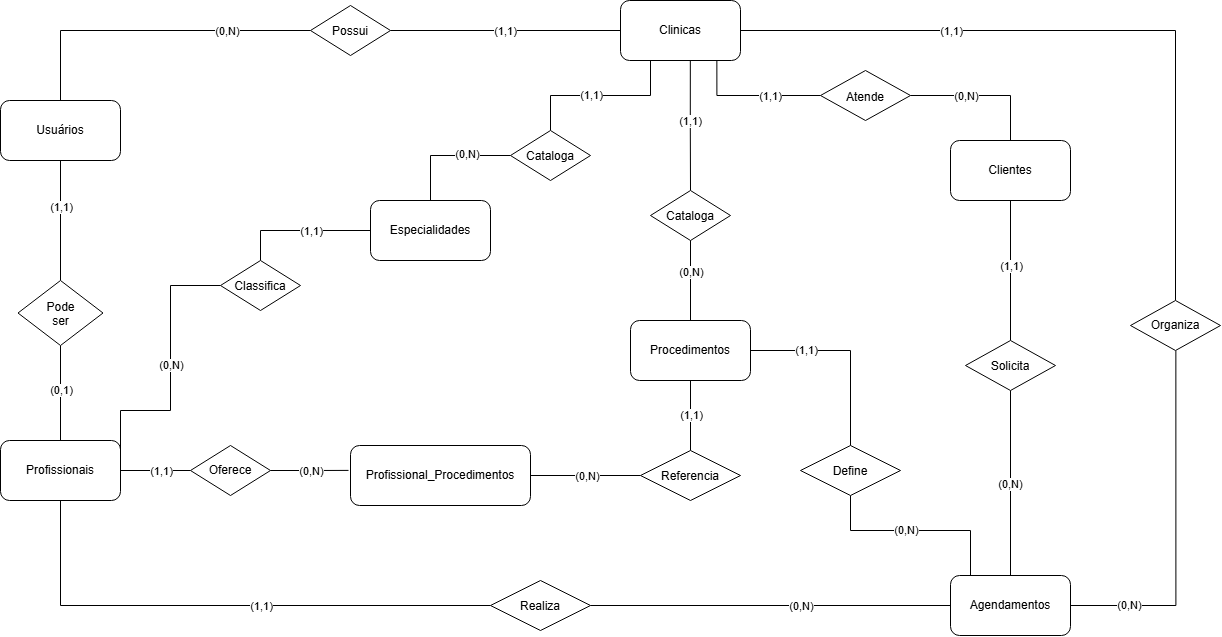
\includegraphics[width=\linewidth,height=0.78\textheight,keepaspectratio]{assets/mer-conceitual-agendai.png}\caption{Modelo entidade-relacionamento do Agend.AI}\label{fig:der}\end{figure}\end{landscape}\subsection{Descrição das tabelas}\begin{center}\footnotesize\begin{tabularx}{\textwidth}{p{4.2cm}Y}\toprule\textbf{Tabela} & \textbf{Descrição} \\\midrule\texttt{clinicas} & Mantém os dados da clínica e as configurações necessárias para integrar sua agenda ao Google Calendar. Também delimita o escopo dos demais cadastros. \\\texttt{usuarios} & Armazena as credenciais, os dados de identificação e o cargo dos usuários vinculados à clínica. \\\texttt{especialidades} & Representa o catálogo de especialidades da clínica e permite classificar os profissionais. \\\texttt{profissionais} & Complementa o cadastro do usuário com sua especialidade e as informações de integração com a agenda externa. \\\texttt{procedimentos} & Mantém o catálogo geral de serviços da clínica, incluindo valor-base e duração estimada. \\\texttt{pro.\_procedimentos} & Relaciona profissionais e procedimentos, registrando quais serviços são oferecidos e seus valores e durações efetivos. \\\texttt{clientes} & Armazena os dados dos pacientes ou clientes atendidos pela clínica, incluindo telefone e identificação no Telegram quando disponível. \\\texttt{agendamentos} & Registra a relação entre clínica, cliente, profissional e procedimento, além do período, valor, situação do atendimento, pagamento e evento correspondente no Google Calendar. \\\bottomrule\end{tabularx}\end{center}As indisponibilidades simples permanecem como eventos do Google Calendar e não exigem uma tabela própria no MVP.

\section{APIs e integrações}

O aplicativo consumirá uma API REST em ASP.NET Core. As rotas utilizadas diretamente pelo aplicativo são apresentadas na Tabela~\ref{tab:apis-mobile}.\begin{table}[H]\centering\caption{APIs utilizadas pelo aplicativo}\label{tab:apis-mobile}\small\begin{tabularx}{\textwidth}{>{\raggedright\arraybackslash}p{7.4cm}Y}\toprule\textbf{Método e rota} & \textbf{Uso no aplicativo} \\\midrule\textbf{POST} \path{/api/auth/login} & Autenticar e obter access token. \\\textbf{GET} \path{/api/me} & Carregar perfil e UUID do profissional autenticado. \\
\textbf{GET} \path{/api/me/overview} & Carregar próximo atendimento e indicadores resumidos da tela inicial. \\\textbf{GET} \path{/api/agenda/\{profissionalUuid\}} & Consultar atendimentos e indisponibilidades no período. \\\textbf{GET} \path{/api/agendamentos/\{agendamentoUuid\}} & Carregar detalhes do atendimento. \\\textbf{POST} \path{/api/me/indisponibilidades} & Criar bloqueio pontual na própria agenda. \\\textbf{DELETE} \path{/api/me/indisponibilidades/\{eventoId\}} & Remover bloqueio pertencente ao profissional. \\\textbf{GET} \path{/api/procedimentos} & Listar catálogo ativo da clínica para seleção. \\\textbf{GET} \path{/api/me/procedimentos} & Listar associações e valores efetivos do profissional. \\\textbf{POST} \path{/api/me/procedimentos} & Associar procedimento existente ao profissional. \\\textbf{PATCH} \path{/api/me/procedimentos/\{profissionalProcedimentoUuid\}} & Alterar valor, duração ou disponibilidade. \\\textbf{GET} \path{/api/me/receitas/resumo} & Obter indicadores financeiros agregados. \\\bottomrule\end{tabularx}\end{table}Os dados serão trafegados em formato JSON por HTTPS. O token de acesso será armazenado de forma segura no Expo SecureStore e enviado no cabeçalho de autorização das requisições. O aplicativo não se comunicará diretamente com o banco de dados, o n8n ou o Google Calendar, pois todas essas integrações serão intermediadas pela API. Caberá à API validar a autenticação, aplicar as regras de autorização e acessar os dados persistidos. Para a criação e consulta de eventos no Google Calendar, a API utilizará o n8n como camada de integração.

\section{Arquitetura do aplicativo}

\begin{figure}[H]\centering\fcolorbox{agendteal}{agendgray}{\begin{minipage}{0.90\textwidth}\footnotesize\texttt{mobile/}\par\texttt{|-- app/}\hfill{\normalfont\footnotesize rotas Expo Router}\par\texttt{\hspace*{1em}|-- (public)/login.tsx}\par\texttt{\hspace*{1em}\textasciigrave{}-- (private)/}\par\texttt{\hspace*{2em}|-- \_layout.tsx}\par\texttt{\hspace*{2em}|-- index.tsx}\par\texttt{\hspace*{2em}|-- agenda/}\par\texttt{\hspace*{2em}|-- receitas.tsx}\par\texttt{\hspace*{2em}|-- procedimentos/}\par\texttt{\hspace*{2em}\textasciigrave{}-- perfil.tsx}\par\texttt{|-- src/}\par\texttt{\hspace*{1em}|-- components/}\hfill{\normalfont\footnotesize componentes reutilizáveis}\par\texttt{\hspace*{1em}|-- features/}\hfill{\normalfont\footnotesize agenda, receitas, procedimentos e autenticação}\par\texttt{\hspace*{1em}|-- services/}\hfill{\normalfont\footnotesize cliente HTTP e contratos da API}\par\texttt{\hspace*{1em}|-- hooks/}\hfill{\normalfont\footnotesize estado e coordenação das telas}\par\texttt{\hspace*{1em}|-- theme/}\hfill{\normalfont\footnotesize cores, tipografia e espaçamentos}\par\texttt{\hspace*{1em}|-- storage/}\hfill{\normalfont\footnotesize acesso ao SecureStore}\par\texttt{\hspace*{1em}|-- types/}\hfill{\normalfont\footnotesize tipos compartilhados}\par\texttt{\hspace*{1em}\textasciigrave{}-- utils/}\hfill{\normalfont\footnotesize data, moeda e validações simples}\par\texttt{\textasciigrave{}-- assets/}\hfill{\normalfont\footnotesize imagens, ícones e fontes locais}\par\end{minipage}}\caption{Estrutura de pastas proposta para o aplicativo mobile}\label{fig:arquitetura}\end{figure}A estrutura separa as rotas do Expo Router das responsabilidades internas do aplicativo. A pasta \texttt{app/} contém apenas rotas e layouts; \texttt{src/features/} organiza autenticação, agenda, receitas e procedimentos; \texttt{src/services/} concentra o cliente HTTP e seus contratos; e \texttt{src/storage/} isola o acesso ao SecureStore. Componentes, hooks, tema, tipos e utilitários permanecem reutilizáveis e independentes das telas. Essa organização por funcionalidades reduz o acoplamento e facilita a evolução do MVP.

% ==========================================================
\chapter{Planejamento de execução}
% ==========================================================

\section{Backlog de tarefas}

As histórias foram priorizadas em P0, indispensáveis para a entrega, e P1, importantes para qualidade.

\begin{table}[H]
\centering
\caption{Backlog priorizado do MVP}
\small
\begin{tabularx}{\textwidth}{C{1.2cm}Y C{1.4cm}}
\toprule
\textbf{ID} & \textbf{História de usuário} & \textbf{Prioridade} \\
\midrule
US01 & Como profissional, quero entrar no aplicativo para acessar meus dados. & P0 \\
US02 & Como profissional, quero visualizar minha agenda para organizar o dia. & P0 \\
US03 & Como profissional, quero abrir um atendimento para consultar seus detalhes. & P0 \\
US04 & Como profissional, quero bloquear ou liberar um horário para controlar minha disponibilidade. & P0 \\
US05 & Como profissional, quero consultar um resumo de receitas para acompanhar meus resultados. & P0 \\
US06 & Como profissional, quero selecionar os procedimentos que ofereço no catálogo da clínica. & P0 \\
US07 & Como profissional, quero editar preço, duração e disponibilidade dos meus procedimentos. & P0 \\
US08 & Como profissional, quero consultar meu perfil e sair da conta com segurança. & P1 \\
US09 & Como usuário, quero receber mensagens claras em carregamentos, vazios e erros. & P1 \\
US10 & Como avaliador, quero executar um fluxo integrado e estável durante a apresentação. & P0 \\
\bottomrule
\end{tabularx}
\end{table}

\section{Cronograma estimado}

\begin{table}[H]
\centering
\caption{Cronograma de implementação}
\small
\begin{tabularx}{\textwidth}{p{3.2cm}Y}
\toprule
\textbf{Período} & \textbf{Atividades} \\
\midrule
30/09 a 06/10 & Criação do projeto Expo, componentes, navegação e autenticação. \\
07/10 a 13/10 & Agenda, navegação por período e detalhes do atendimento. \\
14/10 a 20/10 & Criação e remoção de indisponibilidades pelo Google Calendar. \\
21/10 a 27/10 & Catálogo, procedimentos do profissional e edição de valores. \\
28/10 a 03/11 & Resumo de receitas, perfil e integração das telas. \\
04/11 a 10/11 & Tratamento de erros, acessibilidade e testes dos fluxos principais. \\
11/11 a 17/11 & Correções, build, documentação e preparação da apresentação. \\
\bottomrule
\end{tabularx}
\end{table}

O escopo será congelado durante a implementação. Caso ocorra atraso, serão reduzidos apenas refinamentos de prioridade P1, sem acrescentar funcionalidades futuras ao MVP.

\postextual

\bibliography{referencias}

\end{document}